\chapter{Vision ``GalleryVR''}

Die Vision soll dazu dienen, einen �berblick �ber die Applikation zu geben, die im Rahmen der Bachelorarbeit erstellt wird.

\section{Problemstellung}

Es soll eine Applikation, ``GalleryVR'', entwickelt werden, welche Gebrauch von der Oculus Rift macht, um die Bilder und die Musik des Anwenders ansprechend darzustellen, z.B. in Form eines 3D-Karussels. Die zus�tzliche "Tiefe", die durch den Einsatz eines \gls{hmd} entsteht, soll dem Anwender helfen, sich in seiner Medienbibliothek schneller zurechtzufinden.

Zus�tzlich dazu soll die Leap Motion dazu verwendet werden, um vollst�ndige Handfreiheit zu gew�hren: Der Anwender soll komplett ohne Maus und Tastatur imstande sein, sich durch seine Bilder zu navigieren.

Kurz zusammengefasst muss die Applikation:

\begin{itemize}
	\item Die Bild- und Musikbibliothek des Benutzers in stereoskopischem 3D darstellen.
	\item Diese freih�ndig durchsuchbar machen mit Sortier- und Gruppierfunktion.
	\item Die Bilder betrachtbar und die Musik abspielbar machen.
	\item Metainformationen darstellen (z.B. in Form von Diagrammen).
\end{itemize}


\section{Technologien}

Das Projekt verwendet spezielle Hardware und Software. Es folgt eine kurze Erkl�rung zu diesen Technologien.

\subsection{Oculus Rift}

Die Oculus Rift ist ein stereoskopisches \gls{hmd}, welches durch Oculus VR entwickelt wird. Die aktuelle Version ist das Developer Kit 2 (DK2). Ein Termin f�r die finale Version steht noch nicht fest.

Hardwarem�ssig besteht die Rift aus einem Headset f�r das Bild und einer Kamera f�r das Head-Tracking. Das Headset wird per USB und HDMI an den Computer angeschlossen und �ber ein Stromkabel mit Strom versorgt. Die Kamera wird auf dem Computerbildschirm platziert, und per USB an den Computer und per Sync-Kabel an die Rift angeschlossen.

\begin{figure}[h]
\centering
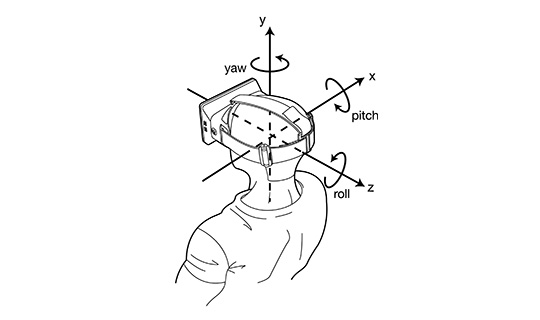
\includegraphics[width=0.7\linewidth]{bilder/rift1}
\caption{Illustration, welche die Anwendung und das Koordinatensystem der Oculus Rift verdeutlicht.}
\floatfoot{Quelle: \url{https://www.oculus.com/blog/building-a-sensor-for-low-latency-vr/}}
\label{fig:rift1}
\end{figure}


Seit DK2 ist das Headset mit 40 Infrarot-LEDs best�ckt, welche mit einer bestimmten Frequenz aufleuchten und von der Kamera f�r das Head-Tracking benutzt werden.
 
Auf der Software-Seite wird ein Treiber auf dem Computer installiert, der nach einer Registration als Entwickler auf der offiziellen Seite erh�ltlich ist . Die Software erlaubt die Erstellung von Benutzerprofilen, um die \gls{ipd} korrekt einzustellen. Es ist ausserdem m�glich, zwischen zwei Betriebsmodi auszuw�hlen: dem traditionellen Modus, wo die Rift als zweiter Bildschirm angesprochen wird, und dem neuen ``Direct Mode'', wo die Rift direkt angesprochen wird.

\subsection{Leap Motion}

Die Leap Motion besteht aus einem rechteckigen Ger�t mit zwei Infrarotsensoren, welche deren Daten per USB auf den angeschlossenen Computer �bertr�gt. Nach der Installation der Leap Motion Runtime l�uft auf dem Computer ein Service, der diese Daten empf�ngt, verarbeitet und per API mit einer variablen Framerate verschiedenen Applikationen zur Verf�gung stellt.

Die Daten, welche diese API liefert, sind in sogenannte ``Frames'' gruppiert. Ein Frame ist sozusagen eine Momentaufnahme der Realit�t, welche sich aus erkannten H�nden zusammensetzt. Durchschnittlich werden pro Sekunde etwa um die 100 dieser Frames berechnet.

\begin{figure}[H]
	\centering
	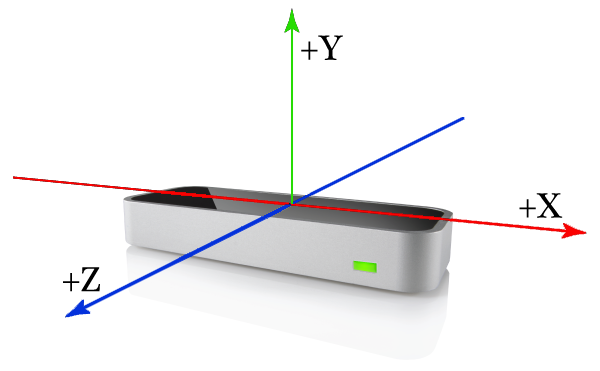
\includegraphics[width=0.7\linewidth]{bilder/leap1}
	\caption{Verdeutlichung des Koordinatensystems.}
	\floatfoot{Quelle: \url{https://developer.leapmotion.com/documentation/csharp/devguide/Leap_Coordinate_Mapping.html}}
	\label{fig:leap1}
\end{figure}

Durch diese Frames kann man auf die Daten der H�nde zugreifen. Jede Hand erh�lt eine ID, womit man gleiche H�nde Frame-�bergreifend identifizieren kann, sowie die dazugeh�renden Koordinaten und Drehungen. Auf Abbildung 2 wird ersichtlich, dass sich die Koordinaten in einem rechtsh�ndigen Koordinatensystem befinden, wobei die Y-Achse nach oben zeigt und die Masse in Millimeter angegeben sind. Die Koordinaten der Finger sind innerhalb von Finger-Instanzen gruppiert, welche wiederum ihre Gelenke als Instanzen einer Joint-Klasse zur Verf�gung stellen.

\begin{figure}[h]
	\centering
	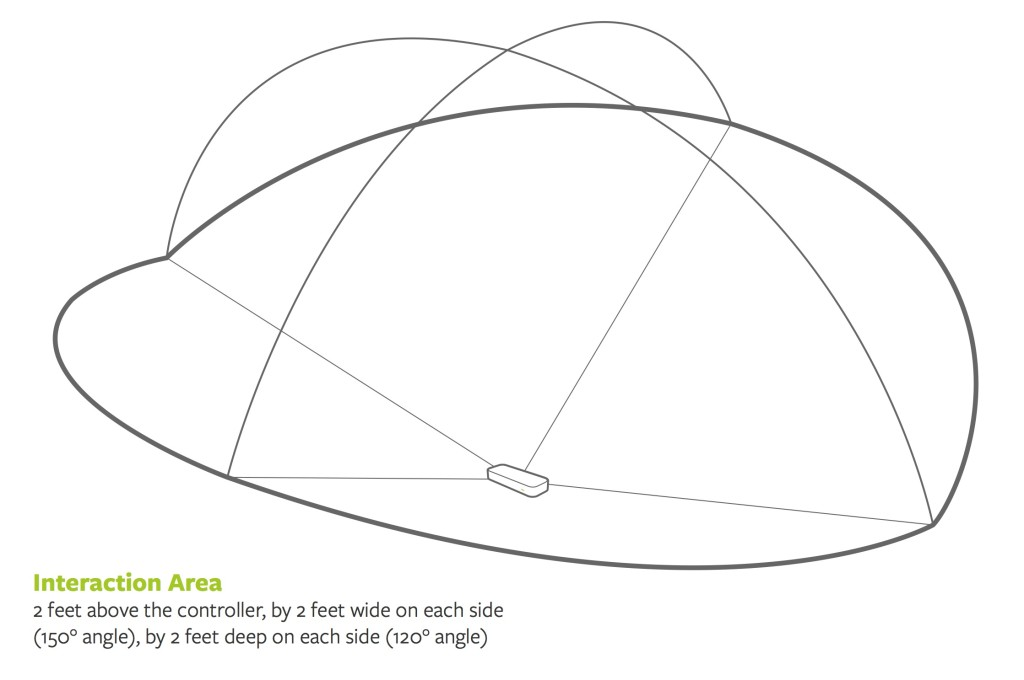
\includegraphics[width=0.7\linewidth]{bilder/leap2}
	\caption{Das Sichtfeld der Leap Motion.}
	\floatfoot{Quelle: \url{https://community.leapmotion.com/t/accurately-measuring-distances/842/3 }}
	\label{fig:leap2}
\end{figure}

Die Leap Motion hat ungef�hr eine Reichweite von einem Meter, wobei das Interaktionsfeld einer Form, wie in Abbildung 3 ersichtlich ist, entspricht. Das Sichtfeld liegt bei 150� in vertikaler und 120� in horizontaler Richtung.


\subsection{Unity 5}

Unity ist eine Entwicklungsumgebung und eine Spiel-Engine, die momentan aufgrund ihrer Bedienungsfreundlichkeit und einer frei erh�ltlichen Version sehr beliebt in der Szene der Indie-Developer ist. Gleichzeitig dient sie auch als gutes Prototyping-Tool, um schnell Ideen umzusetzen.

Am 3. M�rz 2015 machte Unity einen Versionssprung und ist nun als Unity 5 erh�ltlich. Neben anderen Neuerungen sind jetzt alle Funktionen, f�r die fr�her eine kostenpflichtige Lizenz erworben werden musste, auch in der freien Version erh�ltlich, was auch f�r dieses Projekt einen gr�sseren Spielraum bedeutet.

In diesem Projekt wurde Unity wegen der angenehmen Lernkurve und der guten Integrierung mit der Oculus Rift und der Leap Motion f�r den Einsatz gew�hlt. Wie bereits erw�hnt ist es leicht, schnell zu Ergebnissen zu kommen und die Entwicklungsumgebung verwendet die zwei Programmiersprachen f�r die Entwicklung, die der Verfasser dieses Dokuments am besten beherrscht.